% ****** Start of file apssamp.tex ******
%
%   This file is part of the APS files in the REVTeX 4.2 distribution.
%   Version 4.2a of REVTeX, December 2014
%
%   Copyright (c) 2014 The American Physical Society.
%
%   See the REVTeX 4 README file for restrictions and more information.
%
% TeX'ing this file requires that you have AMS-LaTeX 2.0 installed
% as well as the rest of the prerequisites for REVTeX 4.2
%
% See the REVTeX 4 README file
% It also requires running BibTeX. The commands are as follows:
%
%  1)  latex apssamp.tex
%  2)  bibtex apssamp
%  3)  latex apssamp.tex
%  4)  latex apssamp.tex
%
\documentclass[%
 reprint,
 amsmath,amssymb,
 aps,
floatfix,
]{revtex4-2}

\usepackage{graphicx}% Include figure files
\usepackage{dcolumn}% Align table columns on decimal point
\usepackage{bm}% bold math
\usepackage{amsmath}
\usepackage{verbatim} 

\begin{document}

\title{Using the Fourier transform to identify the lag/position between identical signals}% Force line breaks with \\
\date{\today}

\maketitle

\section{Background}
The Fast Fourier Transform (FFT) can be used to quickly identify the lag between two identical one-dimensional (1D) signals, or to find a smaller image which is contained in a bigger image which is the lag in two dimensions(2D).

The steps to identify the lag between two signals $s1$ and $s2$ is:

\begin{enumerate}
    \item Take the FFT of $s_1(t)$ and $s_2(t)$ over time $t$ to create the transformed vectors $\hat{s_1}(\omega)$ and $\hat{s_2}(\omega)$ for frequencies $\omega$.
    \item Take the negative conjugate of one of the signals, say $\hat{s_2}(\omega)\rightarrow-\overline{\hat{s_2}(\omega)}$.
    \item Point-wise multiply $\hat{s_1}(\omega)$ and $-\overline{\hat{s_2}(\omega)}$: -$\hat{s_1}(\omega).\overline{\hat{s_2}(\omega)}$.
    \item Take the inverse FFT to get the lag.
\end{enumerate}

\subsection{Deriving the lag between two identical 1D signals}
I start by deriving the time-shift property of the Fourier Transform (FT), then use to show the steps above work.

\subsubsection{Time-shift property of the Fourier transform}
The FT acts on a signal $f(t)$ via the operator $\mathcal{F}$ such that a function over time $f(t)$ is mapped onto frequency space $\hat{\chi}(\omega)$:

\begin{align}
    \mathcal{F}\{f(t)\} &= \int^{\infty}_{-\infty} f(t)e^{-i\omega t}\,dt \\
    \label{eqn:FFT}
    &= \hat{\chi}(\omega).
\end{align}

Now introduce a time-shift $t-t_0$ to Eqn.~\ref{eqn:FFT} and use a change of variables to obtain the time-shift property:

\begin{align}
    \mathcal{F}\{f(t-t_0)\} &= \int^{\infty}_{-\infty} f(t-t_0)e^{-i\omega t}\,dt \label{eqn:FFT_shift1} \\
    &= \int^{\infty}_{-\infty} f(u)e^{-i\omega (u+t_0)}\,du\label{eqn:FFT_shift2}\\ 
    & \mathrm{where}\: u=t-t_0 \nonumber \\
    &= e^{-i\omega t_0}\int^{\infty}_{-\infty} f(u)e^{-i\omega u}\,du\label{eqn:FFT_shift3}\\ 
    &= e^{-i\omega t_0}\hat{\chi}(\omega).\label{eqn:FFT_shift4}
\end{align} 

\subsubsection{Obtaining the lag between two identical 1D signals}
Using Eqn.~\ref{eqn:FFT_shift4} and following the steps outlined above we start with two signals $f_1(t)$ and $f_2(t)$ where $f_2(t)=f_1(t-t_0)$.

\textbf{Step 1:} Transform $f_1(t)$ and $f_2(t)$ into frequency space: 
\begin{align}
    \mathcal{F}\{f_1(t)\} &= \hat{\chi}_1(\omega),\label{eqn:sig_2a}
\end{align}

and

\begin{align}
    \mathcal{F}\{f_2(t)\} &= \hat{\chi}_2(\omega)\nonumber \\
    &= e^{-i\omega t_0}\hat{\chi}_1(\omega).\label{eqn:sig_2b}
\end{align}

Where Eqn.~\ref{eqn:sig_2b} is due to the time-shift property of the Fourier transform.

\textbf{Step 2:} Next take negative complex conjugate of one of the signals (say $\hat{\chi}_1(\omega)$) in Eqn.~\ref{eqn:sig_2a} and multiply by Eqn.~\ref{eqn:sig_2b}:

\begin{align}
    \hat{\chi}_2(\omega)\hat{\chi}_1^{*}(\omega)&=
    e^{-i\omega t_0}\hat{\chi}_1(\omega)\hat{\chi}_1^{*}(\omega)\\
    &\mathrm{(time-shift\:property)}\nonumber\\
    &=e^{-i\omega t_0}|\hat{\chi}_1(\omega)|^2\label{eqn:sig_4}\\
    &\mathrm{(modulus\:of\:a\:complex\:function)}\nonumber\\
    &=e^{-i\omega t_0}E_1(\omega)\\
    &\mathrm{(definition\: of\: energy\: spectral\: density)}\nonumber\\
    &=\int^{\infty}_{\infty} e^{-i\omega t_0}|f_{1}(t)|^{2}\,dt,\\
    &\mathrm{(definition\: of\: energy\: spectral\: density)}\nonumber
\end{align}

where $E_1(\omega)$ is the energy spectral density of $\hat{\chi}(\omega)$ and is equal to $E_1(t)$.

\textbf{Step 3:} Now applying the inverse FT operator $\mathcal{F}^{-1}$, we have:
\begin{align}
    &\mathcal{F}^{-1}\left\{\int^{\infty}_{\infty} e^{-i\omega t_0}f_{1}(t)\,dt\right\}= \\
    &\int_{-\infty}^{\infty}\int^{\infty}_{\infty} e^{-i\omega t_0}|f_{1}(t)|^{2}\,dt\: e^{i\omega t'} d\omega. \\
\end{align}

Separating out the integrals:
\begin{align}
    \int_{-\infty}^{\infty} |f_{1}(t)|^{2}\,dt\, \int_{-\infty}^{\infty} e^{-i\omega (t'-t_0)} d\omega. \\
    =E_1(t)\,\delta(t-t_0),\label{eqn:delta}
\end{align}

where:

\begin{align}
    \int_{-\infty}^{\infty} e^{-i\omega (t'-t_0)} d\omega = \delta(t-t_0).
\end{align}

The $\delta$-function in Eqn.~\ref{eqn:delta} means the result is zero everywhere except when $t=t_0$ and thus the maximum (or first non-zero) result is the lag.

\section{Deriving the lag between two identical multi-dimensional signals}

\section{Approach}

\subsection{1D signal matching}
The 1D signals are loaded using the function \texttt{LoadSensorData} and I make sure they are the same size with the function \texttt{MakeSameSize}, and the 1D lag is returned using the function \texttt{Get1DLag} which acts on two input signals.

Looking at \texttt{Get1DLag} in greater detail, this function takes four inputs:

\begin{itemize}
    \item \texttt{signal\_1} - a 1D signal,
    \item \texttt{signal\_2} - an identical 1D signal, which lags behind/ahead of \texttt{signal\_1},
    \item \texttt{sampling\_rate=44100} - the sampling rate given in Hz
    \item \texttt{speed\_sound=333} - the speed of sound in $\mathrm{m.s^{-2}}$.
\end{itemize}

The function returns three outputs in a tuple:

\begin{itemize}
    \item {The number of samples between \texttt{signal\_1} and \texttt{signal\_2} (\texttt{s2\_point\_lag}).}
    \item {The time between \texttt{signal\_1} and \texttt{signal\_2} (\texttt{s2\_time\_lag}).}
    \item {The distance between the two sensors recording \texttt{signal\_1} and \texttt{signal\_2}} (\texttt{distance}).
\end{itemize}

In order to return \texttt{s2\_point\_lag}, \texttt{s2\_time\_lag} and \texttt{distance}, the following steps are taken:

\begin{enumerate}
    \item The two input signals \texttt{signal\_1} and \texttt{signal\_2} are transformed into the frequency domain using the function \texttt{Get1DFFT}, e.g. \texttt{signal\_f, s1=Get1DFFT(signal\_1)} returns the frequency values \texttt{signal\_f} and FT values \texttt{s1} from the recorded signal amplitude \texttt{signal\_1}.
    \item One of the signals is conjugated, here it's \texttt{s1}: \texttt{s1\_conj= -s1.conjugate()}
    \item Next I calculate the lag by multiplying \texttt{s1\_conj} and \texttt{s2}, taking the inverse FT (\texttt{np.fft.ifft}) then finding the maximum:  \texttt{s2\_point\_lag=}\\\texttt{np.argmax(np.abs(np.fft.ifft(s1\_conj*s2)))}.
    \item The lag given is either how much the one signal is ahead \textit{or} behind another. To tell the difference I check if the first/last point of \texttt{signal\_1} matches the lag in \texttt{signal\_2}, which is done by checking \texttt{signal\_1[0]==signal\_2[s2\_point\_lag]} and\\ \texttt{signal\_1[-1:]==signal\_2[s2\_point\_lag-1:s2\_point\_lag]} respectively.
\end{enumerate}

\subsection{2D signal matching}




% \begin{figure}
%      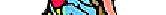
\includegraphics[width=8cm]{rocketman_slice.pdf}
%      \caption{A ten pixel thick slice of Rocketman for illustrative purposes. I only take a one-pixel slice in my approach which would be difficult to see here.}
%      \label{fig:rocketman_slice}
% \end{figure}

\section{Results}


\section{Improvements}


\end{document}
